\documentclass[12pt, a4paper]{article}
\usepackage[spanish]{babel}
\usepackage[utf8]{inputenc}
\usepackage{graphicx}
\usepackage{hyperref}
\usepackage{enumitem}
\usepackage{parskip}
\usepackage{float}
\usepackage{titling}
\usepackage{listings} % Paquete para mostrar código
\usepackage{xcolor} % Paquete para colores en el código

% Configuración personalizada para JavaScript
\lstdefinelanguage{JavaScript}{
    keywords={break, case, catch, continue, debugger, default, delete, do, else, false, finally, for, function, if, in, instanceof, new, null, return, switch, this, throw, true, try, typeof, var, void, while, with, let, const, await, async},
    keywordstyle=\color{blue}\bfseries,
    ndkeywords={class, export, boolean, throw, implements, import, this},
    ndkeywordstyle=\color{darkgray}\bfseries,
    identifierstyle=\color{black},
    sensitive=false,
    comment=[l]{//},
    morecomment=[s]{/*}{*/},
    commentstyle=\color{gray}\ttfamily,
    stringstyle=\color{red}\ttfamily,
    morestring=[b]',
    morestring=[b]"
}

% Configuración del estilo para mostrar código
\lstset{
    language=JavaScript, % Usar el lenguaje definido arriba
    basicstyle=\ttfamily\small, % Fuente monoespaciada y tamaño pequeño
    keywordstyle=\color{blue}, % Color para palabras clave
    stringstyle=\color{red}, % Color para cadenas de texto
    commentstyle=\color{gray}, % Color para comentarios
    breaklines=true, % Permitir saltos de línea
    frame=single, % Agregar un marco alrededor del código
    numbers=left, % Mostrar números de línea a la izquierda
    numberstyle=\tiny\color{gray}, % Estilo de los números de línea
    tabsize=2, % Tamaño de tabulación
    showstringspaces=false % No mostrar espacios en cadenas
}


\title{Informe Técnico: Plataforma Fintrax}
\author{Carlos Ulloa, Patricio Valdés, Víctor Sepúlveda}
\date{Junio 2025}

\begin{document}

\begin{titlepage}
    \maketitle
    \thispagestyle{empty} % Elimina el número en la portada
\end{titlepage}
\newpage
\tableofcontents
\thispagestyle{empty} % Elimina el número en la página del índice
\newpage
\section{Introducción}
Fintrax es una plataforma integral diseñada para el control de ingresos y egresos por proyecto, dirigida a emprendedores, freelancers, startups y organizaciones que requieren una gestión financiera precisa desde etapas tempranas. Este informe detalla las funcionalidades, metodología de desarrollo, arquitectura, y contribuciones individuales del equipo.
\newpage
% Insertamos Metas para el Avance
\section{Meta de Avance Propuesta al Inicio}

\subsection*{Metas Iniciales}
El proyecto Fintrax tiene como objetivo principal desarrollar una plataforma para el control de ingresos y egresos por proyecto, dirigida a emprendedores y organizaciones. Las metas iniciales propuestas incluyen:
\begin{itemize}
    \item Implementar una base de datos estructurada para gestionar proyectos, transacciones, reportes, usuarios y notificaciones.
    \item Desarrollar un frontend interactivo utilizando React.js para facilitar la gestión financiera.
    \item Integrar Supabase como backend para autenticación, almacenamiento y funciones avanzadas como triggers y vistas.
    \item Crear funcionalidades básicas como:
    \begin{itemize}
        \item Registro y autenticación de usuarios.
        \item Gestión de proyectos y transacciones.
        \item Generación de reportes financieros.
        \item Visualización de datos en tiempo real.
    \end{itemize}
\end{itemize}

\subsection*{Avance Actual}
Hasta el momento, se han completado las siguientes tareas:
\begin{itemize}
    \item \textbf{Base de datos:}
    \begin{itemize}
        \item Creación de tablas principales como \texttt{projects}, \texttt{transactions}, \texttt{reports}, \texttt{notifications}, entre otras.
        \item Implementación de Row Level Security (RLS) para garantizar la seguridad de los datos.
        \item Configuración de triggers para auditoría, validaciones y actualizaciones automáticas.
        \item Creación de vistas para facilitar consultas como balances de proyectos y transacciones activas.
    \end{itemize}
    \item \textbf{Backend:}
    \begin{itemize}
        \item Desarrollo de funciones RPC para cálculos financieros y generación de reportes.
        \item Configuración de endpoints para interactuar con la base de datos.
    \end{itemize}
    \item \textbf{Frontend:}
    \begin{itemize}
        \item Implementación de componentes principales como \texttt{Proyectos}, \texttt{Ingresos}, \texttt{Egresos}, \texttt{Reportes}, y \texttt{Perfil}.
        \item Integración de Supabase para autenticación y manejo de datos.
        \item Diseño inicial de la interfaz con estilos personalizados.
    \end{itemize}
\end{itemize}

\subsection*{Próximos Pasos}
El enfoque inmediato será:
\begin{itemize}
    \item Completar las funcionalidades faltantes, como filtros avanzados y exportación de reportes.
    \item Realizar pruebas de integración entre el frontend y el backend.
    \item Mejorar la experiencia de usuario mediante ajustes en el diseño y validaciones en tiempo real.
    \item Desplegar la plataforma para pruebas iniciales.
\end{itemize}
% 
% insertamos la infraestructura
\section{Arquitectura e Infraestructura}
\subsection{Diagrama General}

\subsection{Componentes Principales}
\subsubsection{Frontend}
\begin{itemize}
    \item \textbf{Tecnologías}: React.js con TypeScript
    \item \textbf{Bibliotecas principales}:
    \begin{itemize}
        \item Chart.js para visualización de datos financieros
        \item React Hook Form para manejo de formularios
        \item Axios para comunicación con el backend
    \end{itemize}
    \item \textbf{Características}:
    \begin{itemize}
        \item Interfaz responsive con Tailwind CSS
        \item Validaciones en tiempo real
        \item Actualización automática de datos mediante suscripciones
    \end{itemize}
\end{itemize}

\subsubsection{Backend y Base de Datos}
\begin{itemize}
    \item \textbf{Plataforma}: SupaBase (alternativa open-source a Firebase)
    \item \textbf{Componentes}:
    \begin{itemize}
        \item Autenticación con JWT y OAuth
        \item Base de datos PostgreSQL con Row Level Security (RLS)
        \item Almacenamiento para documentos adjuntos
    \end{itemize}
    \item \textbf{Estructura de datos principal}:
    \begin{itemize}
        \item Tabla \texttt{users} para gestión de cuentas
        \item Tabla \texttt{projects} para seguimiento de proyectos
        \item Tabla \texttt{transactions} para registros financieros
        \item Tabla \texttt{audit\_log} para trazabilidad
    \end{itemize}
\end{itemize}

\subsection{Flujo de Datos}
\begin{enumerate}
    \item El usuario interactúa con la interfaz React
    \item Las acciones disparan llamadas a la API de SupaBase
    \item SupaBase procesa las peticiones aplicando políticas RLS
    \item Los datos se almacenan/recuperan de PostgreSQL
    \item Los cambios se notifican al frontend en tiempo real
    \item La interfaz se actualiza reflejando los cambios
\end{enumerate}

\subsection{Security by Design}
\begin{itemize}
    \item \textbf{Autenticación}:
    \begin{itemize}
        \item Tokens JWT con expiración corta
        \item Verificación de email para nuevos registros
        \item Hasheo de contraseñas con algoritmos modernos
    \end{itemize}
    \item \textbf{Autorización}:
    \begin{itemize}
        \item Row Level Security para acceso a datos
        \item Políticas granulares por tipo de recurso
        \item Validación de ownership antes de operaciones
    \end{itemize}
    \item \textbf{Protección de datos}:
    \begin{itemize}
        \item Soft-delete para recuperación de registros
        \item Auditoría completa de cambios
        \item Encriptación de datos sensibles
    \end{itemize}
\end{itemize}

\subsection{Escalabilidad}
\begin{itemize}
    \item Arquitectura serverless que escala automáticamente
    \item Base de datos optimizada con índices para consultas frecuentes
    \item Caché implementado para reportes complejos
    \item Diseño preparado para migración a microservicios si crece la demanda
\end{itemize} % Sin extensión .tex
% 
% insertamos las funciones
\section{Funcionalidades}
\subsection{Gestión de Usuarios}
\begin{itemize}
    \item \textbf{Autenticación} mediante SupaBase Auth:
    \begin{itemize}
        \item Registro con verificación de email
        \item Inicio de sesión con email/contraseña
        \item Cierre de sesión con invalidación de tokens JWT
        \item Sesiones persistentes seguras
    \end{itemize}
    
    \item \textbf{Recuperación de contraseña}:
    \begin{itemize}
        \item Flujo automatizado con SupaBase
        \item Enlaces de recuperación con expiración
        \item Validación de seguridad en el frontend
    \end{itemize}
    
    \item \textbf{Perfil de usuario}:
    \begin{itemize}
        \item Almacenamiento en tabla \texttt{auth.users} de SupaBase
        \item Edición segura de información básica
    \end{itemize}
\end{itemize}

\subsection{Gestión de Ingresos y Egresos}
\begin{itemize}
    \item \textbf{Registro de transacciones}:
    \begin{itemize}
        \item Implementado mediante tablas \texttt{transacciones} en SupaBase
        \item Campos obligatorios: monto, fecha, descripción, categoría, tipo (ingreso/egreso)
        \item Relación con proyectos mediante \texttt{id\_proyecto}
        \item Validación en tiempo real con SupaBase RPC
    \end{itemize}
    
\item \textbf{Edición y eliminación}:
\begin{itemize}
    \item \textbf{Protección de datos}:
    \begin{itemize}
        \item Implementación de Row Level Security (RLS) para restringir acceso
        \item Políticas personalizadas para UPDATE/DELETE en SupaBase
    \end{itemize}
    
\item \textbf{Soft Delete}:
\begin{itemize}
    \item \textbf{Implementación básica}:
    \begin{itemize}
        \item Campo \texttt{deleted\_at} (TIMESTAMPTZ) en tabla \texttt{transacciones}
        \item Valor por defecto NULL (registro activo)
        \item Índice parcial para optimizar queries: \texttt{WHERE deleted\_at IS NULL}
    \end{itemize}
    
    \item \textbf{Eliminación por errores}:
    \begin{itemize}
        \item Columna adicional \texttt{deletion\_reason} (TEXT) con valores:
        \item \quad 'error' - Registro incorrecto
        \item \quad 'normal' - Eliminación estándar
        \item \quad 'duplicado' - Registro repetido
    \end{itemize}
\end{itemize}
    \item \textbf{Histórico de cambios}:
    \begin{itemize}
        \item Tabla \texttt{transacciones\_log} para auditoría
        \item Triggers en SupaBase que registran:
        \begin{itemize}
            \item Usuario que realizó el cambio
            \item Fecha y hora exacta
            \item Valores anteriores (para operaciones UPDATE/DELETE)
        \end{itemize}
    \end{itemize}
    
    \item \textbf{Validaciones}:
    \begin{itemize}
        \item Confirmación en UI para operaciones críticas
        \item Límite de tiempo para reversión de operaciones
    \end{itemize}
\end{itemize}
    
    \item \textbf{Filtrado avanzado}:
    \begin{itemize}
        \item Uso de SupaBase \texttt{select()} con filtros dinámicos
        \item Posibilidad de filtrar por:
        \begin{itemize}
            \item Rango de fechas
            \item Monto mínimo/máximo
            \item Categorías específicas
            \item Proyecto asociado
        \end{itemize}
        \item Paginación para resultados extensos
    \end{itemize}
    
    \item \textbf{Visualización}:
    \begin{itemize}
        \item Tablas interactivas con ordenamiento por columnas
        \item Resúmenes gráficos usando datos de SupaBase
        \item Vista consolidada por periodos (diario, semanal, mensual)
        \item Sincronización en tiempo real con SupaBase subscriptions
    \end{itemize}
    
    \item \textbf{Validaciones}:
    \begin{itemize}
        \item Restricción de tipos de datos a nivel de base de datos
        \item Verificación de consistencia financiera
        \item Prevención de duplicados
    \end{itemize}
\end{itemize}

\subsection{Reportes y Finanzas}
\begin{itemize}
    \item Generación de reportes financieros
    \item Exportación a formatos estándar (Excel/PDF)
    \item Visualización de balances y gráficos
\end{itemize}
 % Sin extensión .tex
% 
% insertamos el como usar las funciones
\section{Uso de las Funcionalidades}

\subsection*{Gestión de Usuarios}
\begin{itemize}
    \item El usuario accede al formulario de registro e ingresa su correo y contraseña. Un correo de verificación es enviado automáticamente.
    \item Para iniciar sesión, el usuario proporciona sus credenciales previamente registradas. Si son válidas, se establece una sesión persistente.
    \item En caso de olvidar la contraseña, el usuario puede solicitar un enlace de recuperación, el cual expirará después de un tiempo definido.
    \item Desde su perfil, el usuario puede editar su información básica, como nombre o imagen, con cambios guardados automáticamente en Supabase.
    \item El último inicio de sesión del usuario se registra automáticamente mediante triggers en la base de datos.
\end{itemize}

\subsection*{Gestión de Ingresos y Egresos}
\begin{itemize}
    \item Desde el panel principal, el usuario puede registrar nuevas transacciones, completando los campos obligatorios como monto, categoría y fecha.
    \item Las transacciones están vinculadas a un proyecto específico mediante su \texttt{project\_id}.
    \item Las validaciones se realizan en tiempo real: si hay datos inválidos, el sistema los detecta antes de enviarlos a la base de datos.
    \item Para editar o eliminar una transacción, el usuario accede a su historial y selecciona la acción deseada. Las operaciones están protegidas por políticas RLS.
    \item En lugar de eliminar físicamente los datos, se aplica un \textit{soft delete} cambiando el valor de \texttt{deleted\_at}. Esto permite recuperar registros si es necesario.
    \item Cada modificación queda registrada en la tabla \texttt{transactions\_log}, lo cual facilita auditorías y revisiones posteriores.
    \item El sistema permite aplicar filtros avanzados para visualizar datos según fechas, categorías, montos o proyectos, utilizando funciones RPC.
    \item Los resultados se muestran en tablas interactivas y gráficos resumidos, con actualizaciones en tiempo real cuando hay nuevos cambios.
\end{itemize}

\subsection*{Reportes y Finanzas}
\begin{itemize}
    \item Desde el menú de reportes, el usuario puede generar balances por periodos determinados (diario, mensual, anual) mediante funciones RPC.
    \item Los resultados pueden exportarse en formatos como Excel o PDF para análisis externo o presentación \textbf{(pendiente)}.
    \item Los gráficos financieros permiten una visualización rápida del estado general de los ingresos y egresos por proyecto.
\end{itemize}

\subsection*{Gestión de Notificaciones}
\begin{itemize}
    \item El usuario recibe notificaciones relacionadas con sus proyectos y transacciones, las cuales se registran en la tabla \texttt{notifications}.
    \item Las notificaciones pueden ser marcadas como leídas mediante una función RPC.
    \item Las notificaciones expiradas se actualizan automáticamente mediante triggers en la base de datos.
\end{itemize}

\subsection*{Gestión de Adjuntos}
\begin{itemize}
    \item El usuario puede subir archivos relacionados con proyectos y transacciones, como facturas o documentos de soporte.
    \item Los adjuntos se validan para garantizar que cumplan con los formatos permitidos (PDF, JPG, PNG).
    \item Los archivos se almacenan en la tabla \texttt{attachments} y pueden ser consultados mediante funciones RPC.
\end{itemize} % Sin extensión .tex
% 
% Insertamos dificultades
\section{Dificultades}

\subsection{Problemas Técnicos}
Durante el desarrollo del proyecto, se enfrentaron varios problemas técnicos que retrasaron el avance esperado:
\begin{itemize}
    \item \textbf{Integración con Supabase:} La configuración inicial presentó dificultades debido a problemas de compatibilidad con las versiones de las bibliotecas utilizadas.
    \item \textbf{Triggers en la base de datos:} Algunos triggers implementados en PostgreSQL generaron errores inesperados, lo que requirió ajustes y pruebas adicionales.
    \item \textbf{Frontend:} La implementación de componentes dinámicos en React.js presentó desafíos relacionados con el manejo de estados y la sincronización en tiempo real.
\end{itemize}

\subsection{Falta de Tiempo}
Además de los problemas técnicos, la falta de tiempo fue un factor determinante que afectó el progreso del proyecto. Esto se debió principalmente a:
\begin{itemize}
    \item \textbf{Carga Académica:} Los días disponibles para avanzar en el proyecto se redujeron significativamente debido a entregas puntuales de otros cursos, lo que limitó el tiempo dedicado al desarrollo.
    \item \textbf{Prioridades Conflictuantes:} La necesidad de cumplir con otras responsabilidades académicas y personales dificultó la planificación y ejecución eficiente de las tareas del proyecto.
\end{itemize}

\subsection{Impacto en el Avance}
Estas dificultades resultaron en un avance más lento de lo esperado, afectando principalmente:
\begin{itemize}
    \item La implementación de funcionalidades avanzadas como filtros dinámicos y exportación de reportes.
    \item La realización de pruebas exhaustivas para garantizar la calidad del sistema.
    \item La preparación del entorno de despliegue para pruebas iniciales.
\end{itemize}

\subsection{Lecciones Aprendidas}
A pesar de los desafíos, se identificaron áreas clave para mejorar en futuros proyectos:
\begin{itemize}
    \item \textbf{Gestión del Tiempo:} Es fundamental establecer un cronograma más detallado y realista, considerando posibles interrupciones externas.
    \item \textbf{Resolución de Problemas Técnicos:} Dedicar más tiempo a la investigación y pruebas iniciales para evitar retrasos durante la implementación.
    \item \textbf{Comunicación y Colaboración:} Mejorar la coordinación entre los miembros del equipo para optimizar el uso del tiempo disponible.
\end{itemize}
% 
% Insertamos Codigo fuente
\section{Código Fuente}

\subsection{Fragmentos Relevantes}
A continuación, se presentan fragmentos de código funcionales que son esenciales para el funcionamiento de la plataforma, junto con una breve explicación de su propósito y funcionamiento.

\subsubsection{Autenticación de Usuarios}
El siguiente código verifica si un usuario está autenticado y redirige al inicio de sesión si no hay una sesión activa:
\begin{lstlisting}[language=JavaScript]
import { useEffect } from 'react';
import { useNavigate } from 'react-router-dom';
import { supabase } from '../connections/endpoints';

const useAuthCheck = () => {
  const navigate = useNavigate();

  useEffect(() => {
    const checkSession = async () => {
      const { data: session } = await supabase.auth.getSession();
      if (!session?.session?.user) {
        navigate('/');
      }
    };

    checkSession();
  }, [navigate]);

  return { logout };
};
\end{lstlisting}
\textbf{Propósito:} Garantizar que solo usuarios autenticados puedan acceder a las funcionalidades de la plataforma.
\newpage
\subsubsection{Gestión de Proyectos}
Este fragmento obtiene los proyectos asociados al usuario autenticado:
\begin{lstlisting}[language=JavaScript]
const fetchProjects = async (userId) => {
  try {
    const data = await endpoints.projects.getById(userId);
    const userProjects = data.filter((project) => project.user_id === userId);
    setProjects(userProjects);
  } catch (error) {
    console.error('Error fetching projects:', error);
    setErrorMessage('Error inesperado al obtener los proyectos.');
  } finally {
    setLoading(false);
  }
};
\end{lstlisting}
\textbf{Propósito:} Recuperar y mostrar los proyectos del usuario en el frontend.

\subsubsection{Generación de Reportes Financieros}
El siguiente código utiliza una función RPC para generar reportes financieros:
\begin{lstlisting}[language=JavaScript]
const generateReport = async (projectId, reportType, startDate, endDate) => {
  const { data, error } = await supabase.rpc('generate_financial_report', {
    project_id: projectId,
    report_type: reportType,
    start_date: startDate,
    end_date: endDate,
  });
  if (error) throw error;
  return data;
};
\end{lstlisting}
\textbf{Propósito:} Generar reportes financieros personalizados basados en los datos de un proyecto.

\subsubsection{Validación de Transacciones en la Base de Datos}
Este trigger en PostgreSQL valida que las transacciones no excedan el presupuesto del proyecto:
\begin{lstlisting}[language=SQL]
CREATE OR REPLACE FUNCTION public.validate_transaction_budget()
RETURNS TRIGGER AS $$
BEGIN
    IF (NEW.type = 'egreso') THEN
        IF (
            SELECT COALESCE(SUM(CASE WHEN type = 'ingreso' THEN amount ELSE -amount END), 0)
            FROM public.transactions
            WHERE project_id = NEW.project_id AND deleted_at IS NULL
        ) < NEW.amount THEN
            RAISE EXCEPTION 'El monto excede el presupuesto del proyecto.';
        END IF;
    END IF;
    RETURN NEW;
END;
$$ LANGUAGE plpgsql;
\end{lstlisting}
\textbf{Propósito:} Garantizar que las transacciones de tipo "egreso" no superen el presupuesto disponible del proyecto.

\subsection{Conclusión}
Estos fragmentos de código representan las funcionalidades clave de la plataforma, desde la autenticación de usuarios hasta la gestión de proyectos y validaciones en la base de datos. Cada uno de ellos contribuye al correcto funcionamiento del sistema y asegura la integridad de los datos.
%
% Insertamos Capturas
\section{Capturas de Pantalla}

\subsection{Pantalla de Inicio}
\begin{figure}[H]
    \centering
    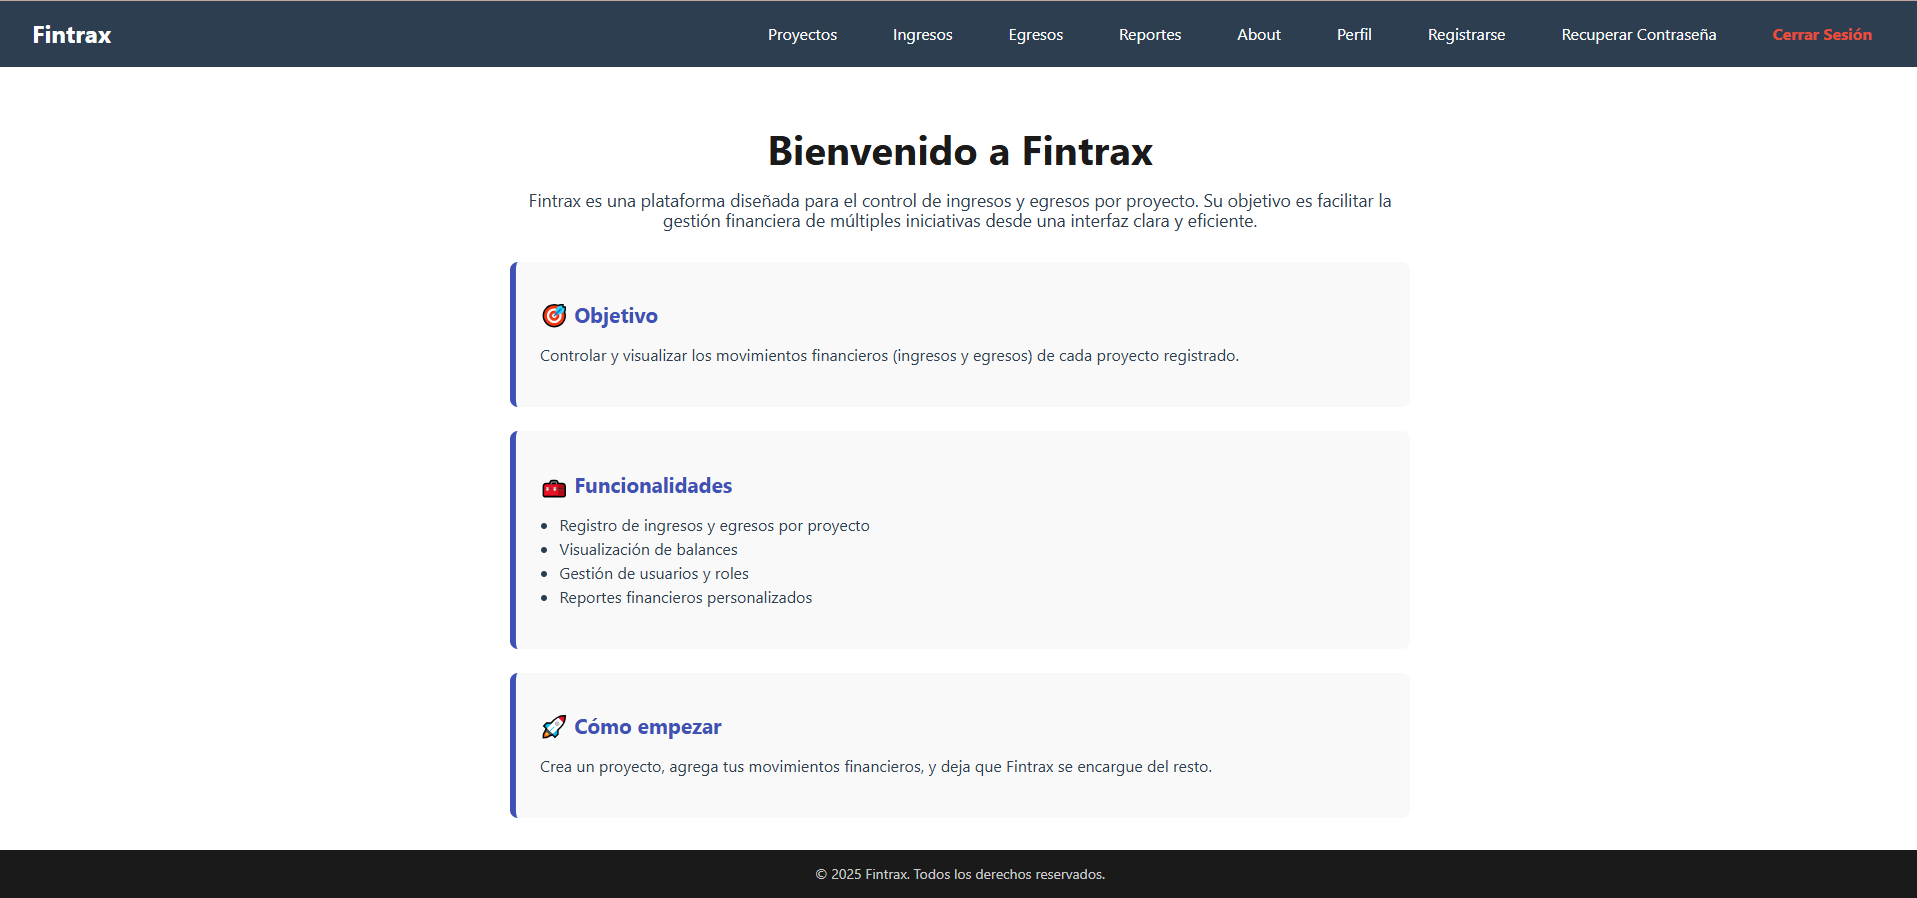
\includegraphics[width=15cm, height=10cm]{Archivos/Capturas/Home.png}
    \caption{Pantalla de Inicio}
    \label{fig:inicio}
\end{figure}

\subsection{Pantalla de Login}
\begin{figure}[H]
    \centering
    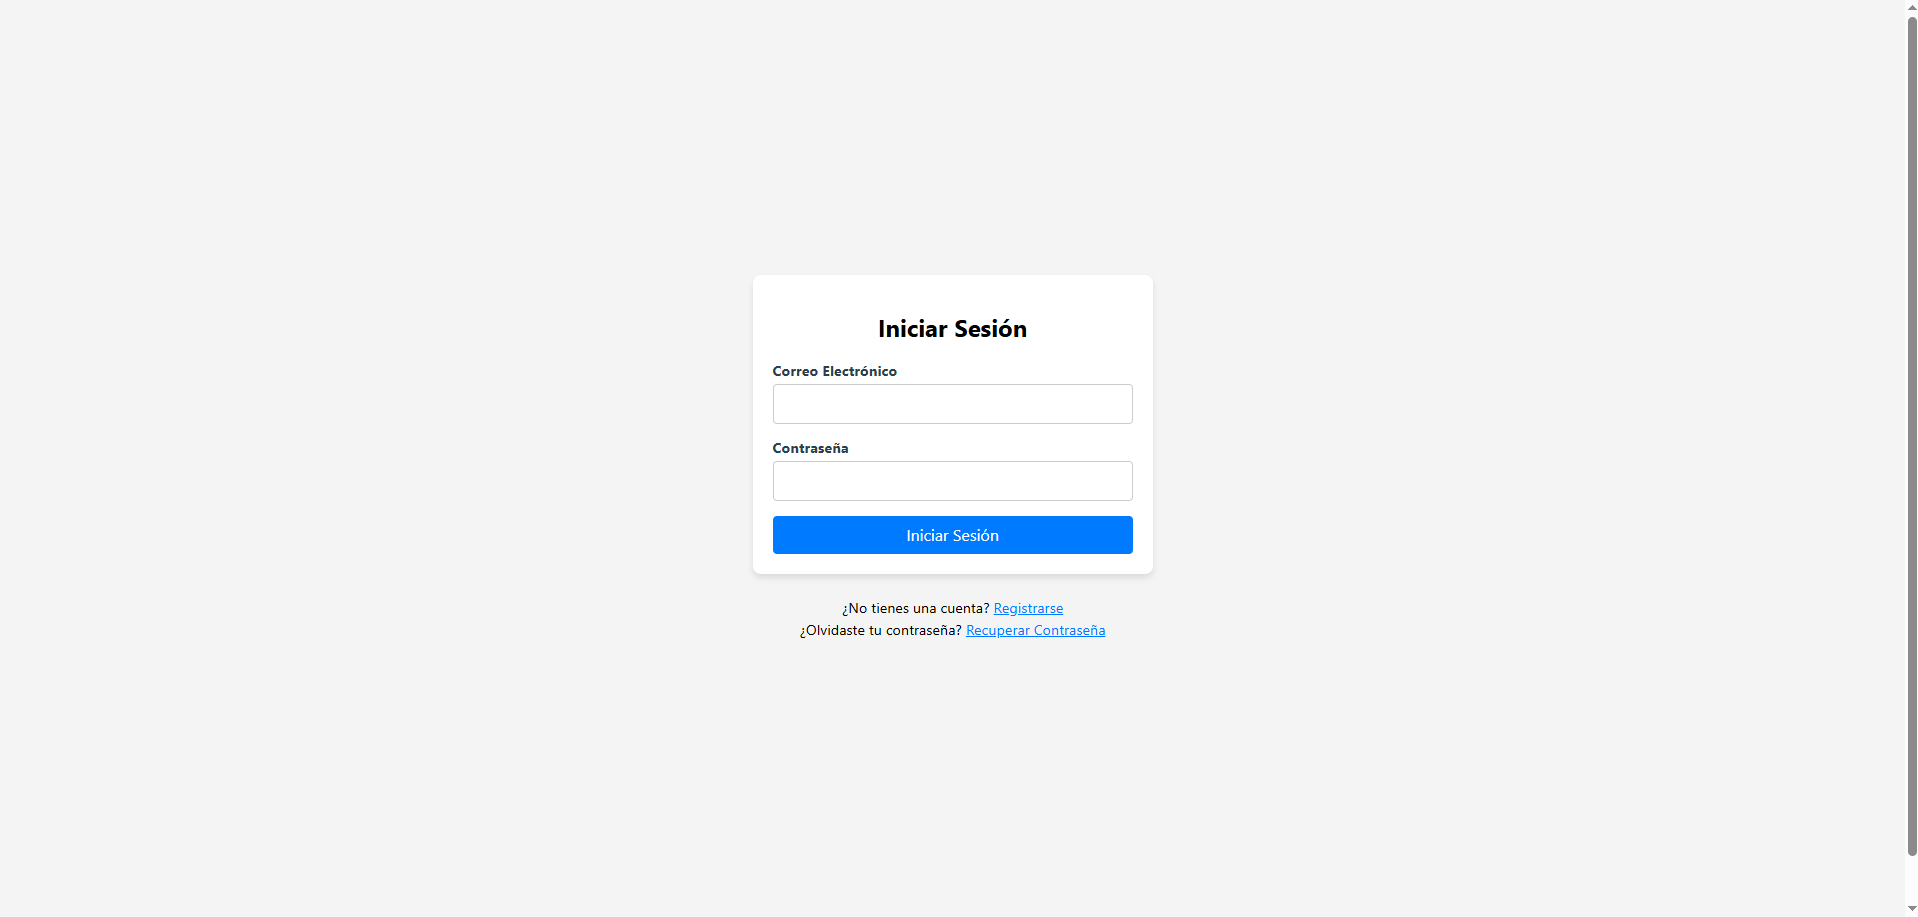
\includegraphics[width=15cm, height=10cm]{Archivos/Capturas/Login.png}
    \caption{Pantalla de Login}
    \label{fig:login}
\end{figure}

\subsection{Pantalla de Perfil}
\begin{figure}[H]
    \centering
    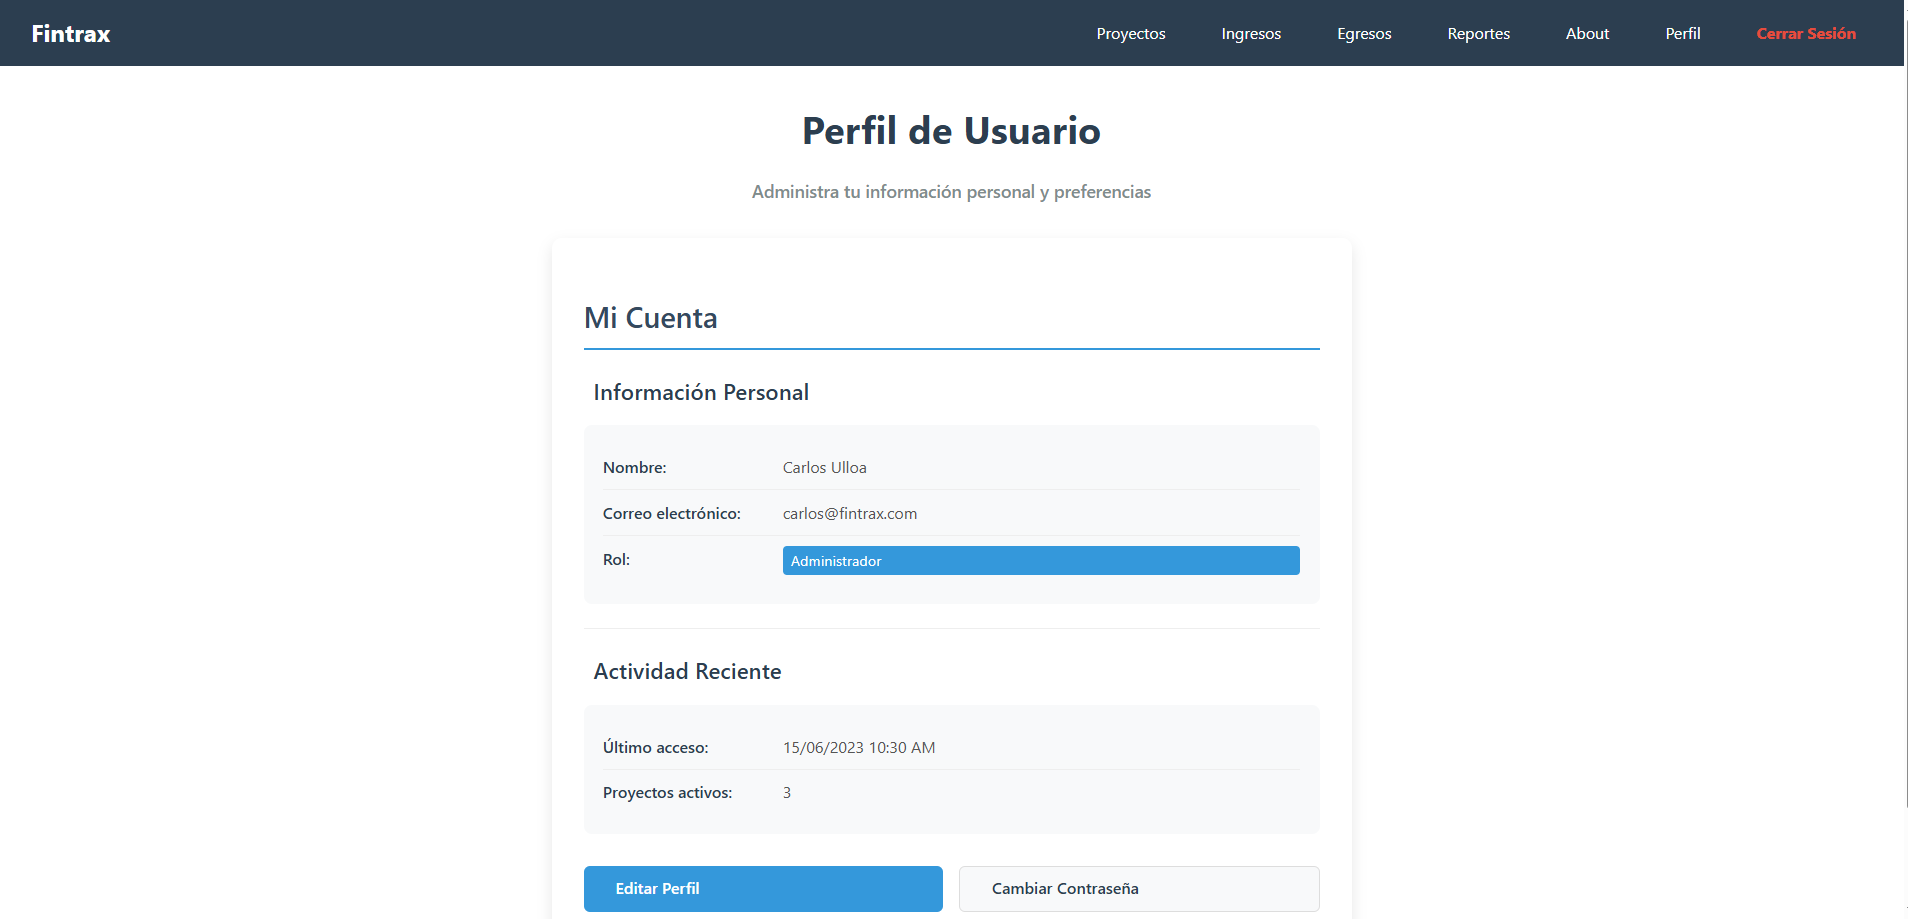
\includegraphics[width=15cm, height=10cm]{Archivos/Capturas/perfil.png}
    \caption{Pantalla de Perfil}
    \label{fig:perfil}
\end{figure}

\subsection{Pantalla de Ingresos}
\begin{figure}[H]
    \centering
    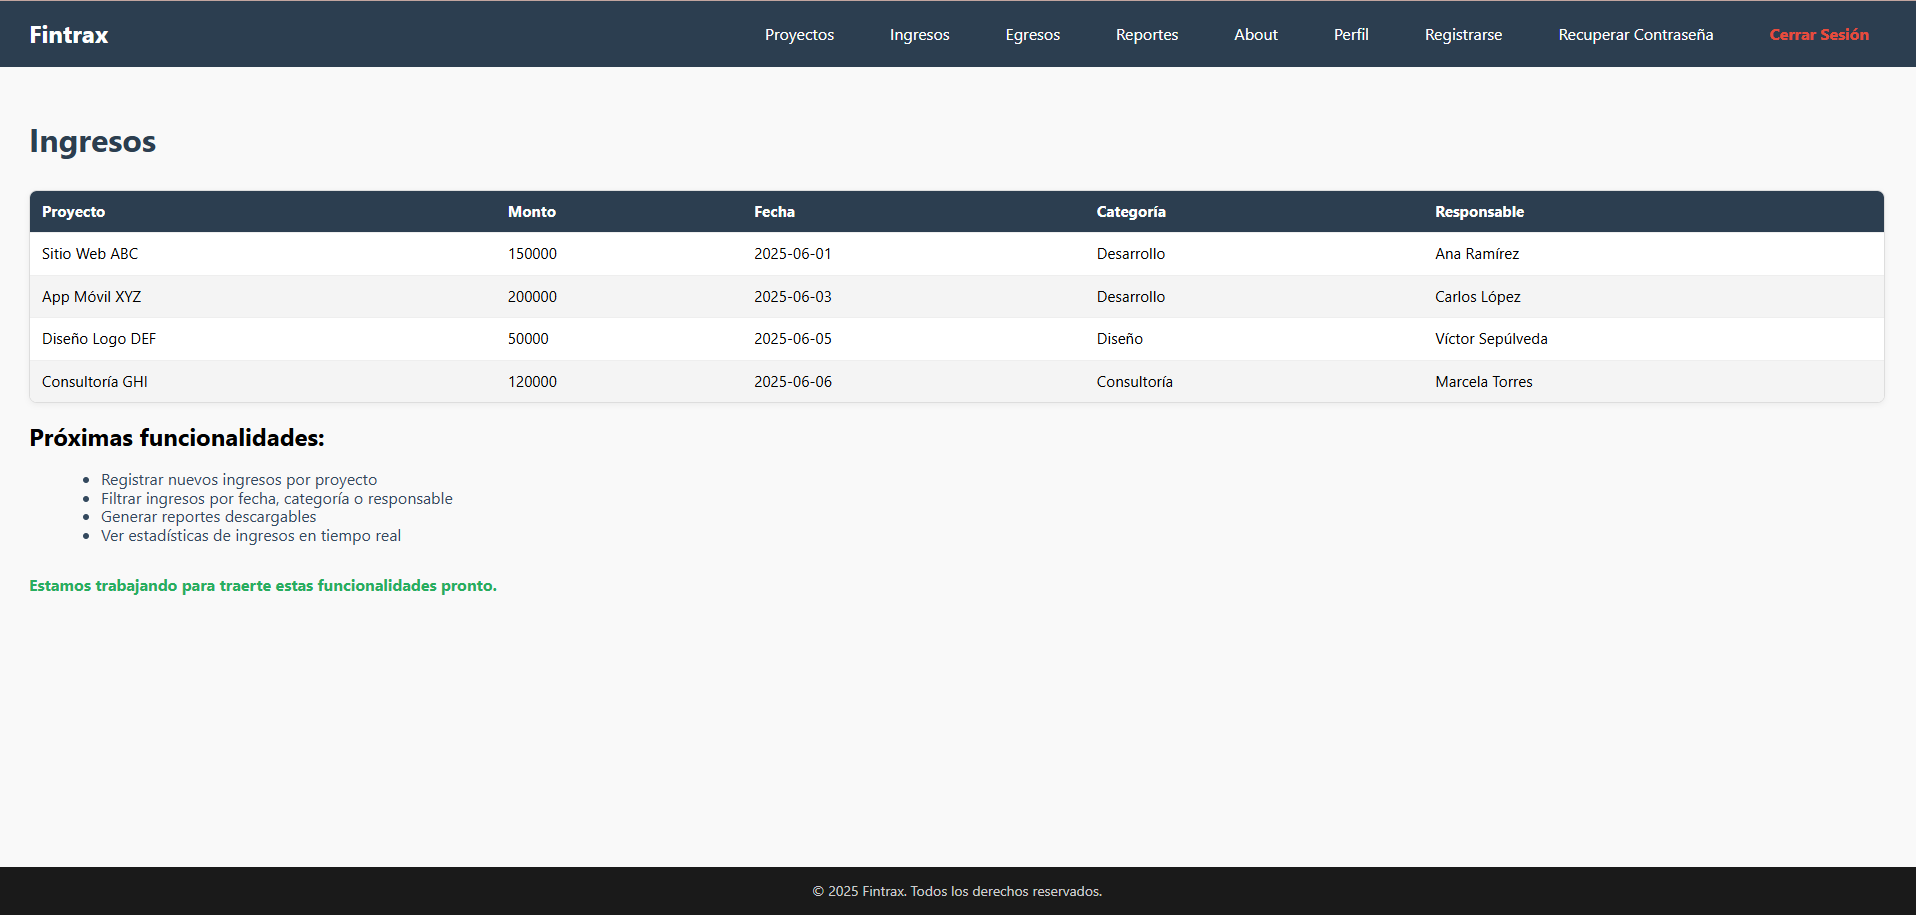
\includegraphics[width=15cm, height=10cm]{Archivos/Capturas/Ingresos.png}
    \caption{Pantalla de Ingresos}
    \label{fig:ingresos}
\end{figure}

\subsection{Pantalla de Egresos}
\begin{figure}[H]
    \centering
    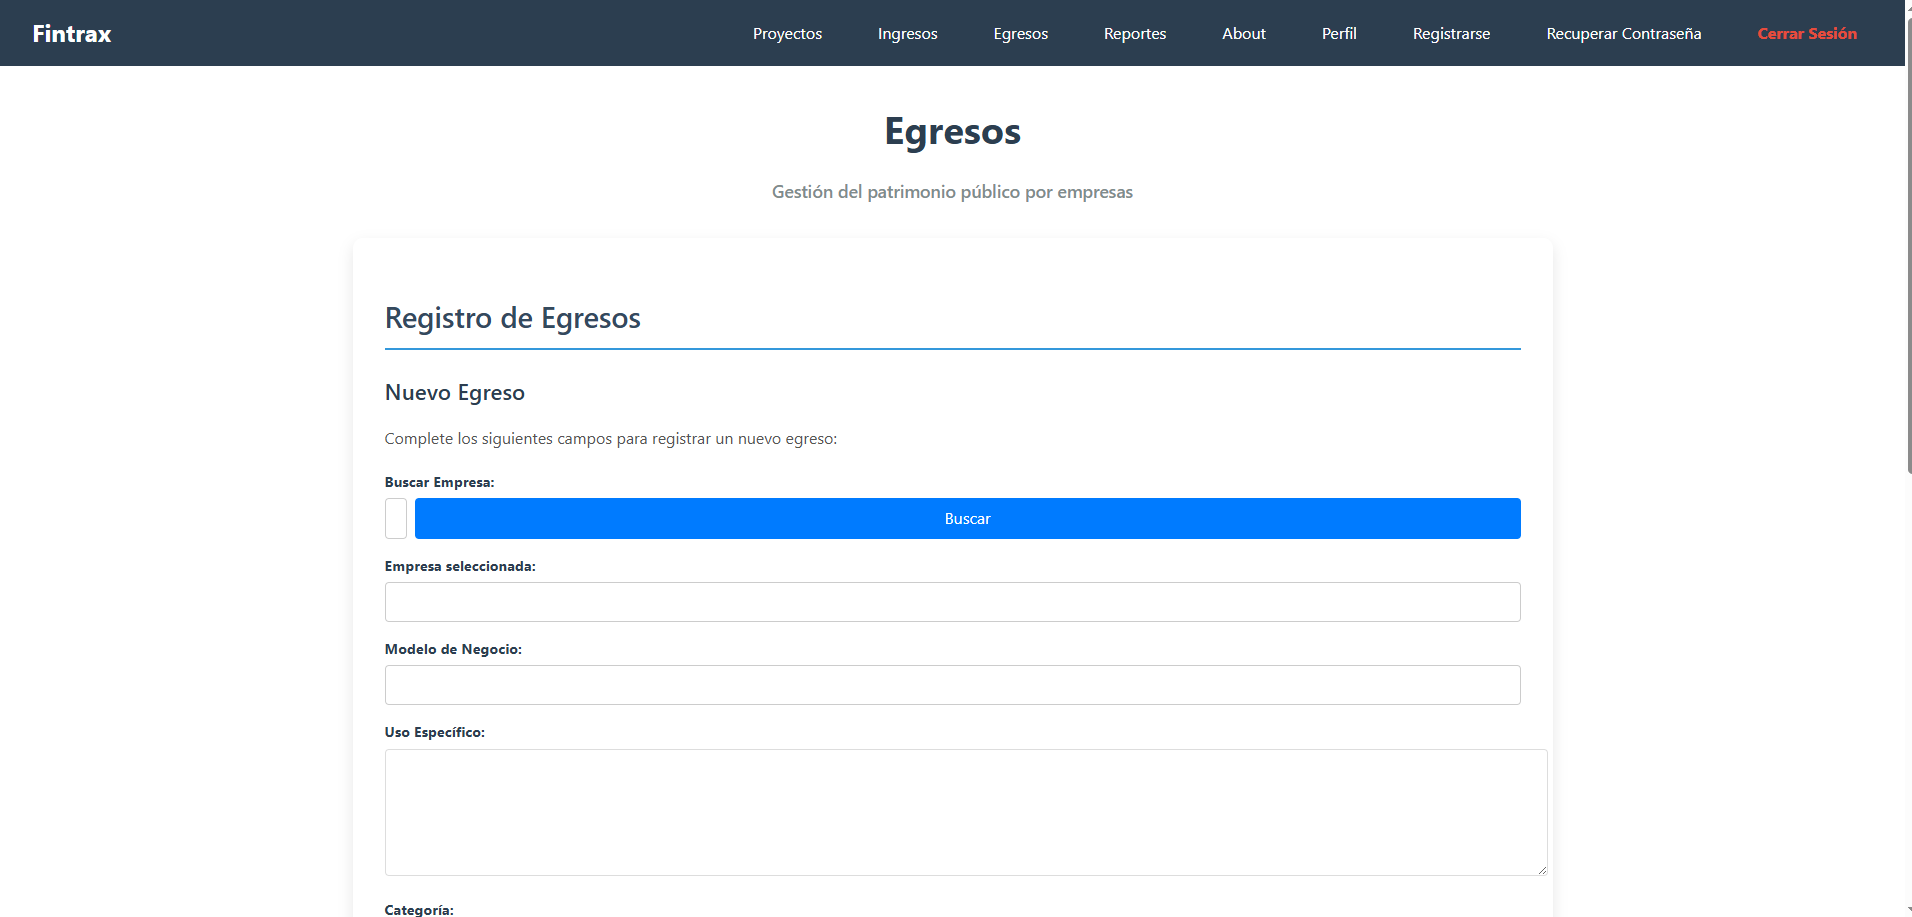
\includegraphics[width=15cm, height=10cm]{Archivos/Capturas/Egresos.png}
    \caption{Pantalla de Egresos}
    \label{fig:egresos}
\end{figure}

\subsection{Pantalla de Reportes}
\begin{figure}[H]
    \centering
    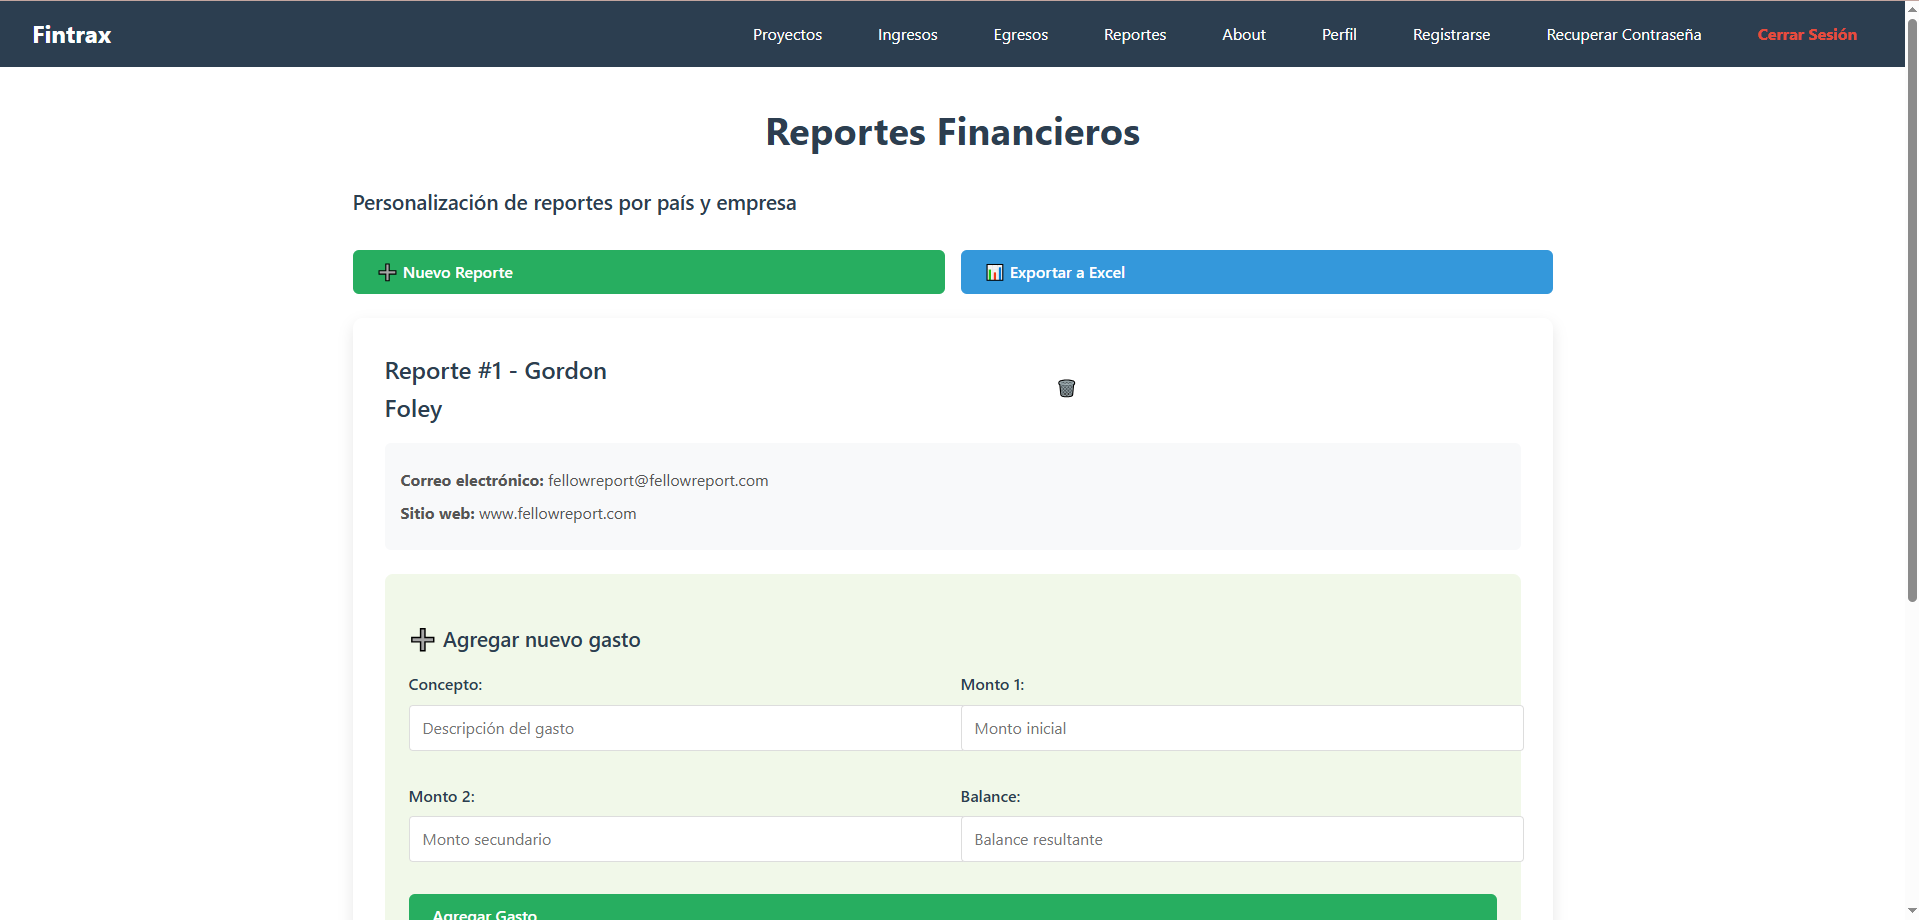
\includegraphics[width=15cm, height=10cm]{Archivos/Capturas/Reportes.png}
    \caption{Pantalla de Reportes}
    \label{fig:reportes}
\end{figure}
% 
% Insertamos Plan de Accion
\section{Plan de Acción para las Próximas Dos Semanas}

\subsection{Objetivos Principales}
Durante las próximas dos semanas, el enfoque estará en completar las funcionalidades faltantes, realizar pruebas de integración y preparar el entorno de despliegue. Los objetivos específicos incluyen:
\begin{itemize}
    \item Implementar filtros avanzados en las vistas de ingresos y egresos.
    \item Agregar funcionalidad de exportación de reportes a Excel y PDF.
    \item Realizar pruebas exhaustivas de integración entre frontend y backend.
    \item Configurar el entorno de despliegue inicial.
\end{itemize}

\subsection{Tareas Detalladas}
\begin{enumerate}
    \item \textbf{Frontend:}
    \begin{itemize}
        \item Implementar filtros avanzados en las vistas de ingresos y egresos.
        \item Agregar funcionalidad de exportación de reportes a Excel y PDF.
        \item Ajustar el diseño para dispositivos móviles.
    \end{itemize}
    \item \textbf{Backend:}
    \begin{itemize}
        \item Implementar pruebas unitarias para las funciones RPC.
        \item Revisar y optimizar índices en la base de datos.
    \end{itemize}
    \item \textbf{Pruebas:}
    \begin{itemize}
        \item Realizar pruebas de integración entre frontend y backend.
        \item Identificar y corregir errores en la interacción entre componentes.
    \end{itemize}
    \item \textbf{Despliegue:}
    \begin{itemize}
        \item Configurar el entorno de despliegue inicial.
        \item Preparar documentación para usuarios y desarrolladores.
    \end{itemize}
\end{enumerate}

\subsection{Cronograma}
\begin{itemize}
    \item \textbf{Semana 1:}
    \begin{itemize}
        \item Implementar filtros avanzados y funcionalidad de exportación en el frontend.
        \item Revisar y optimizar la base de datos.
    \end{itemize}
    \item \textbf{Semana 2:}
    \begin{itemize}
        \item Realizar pruebas de integración y corregir errores.
        \item Configurar el entorno de despliegue y preparar documentación.
    \end{itemize}
\end{itemize}
%  
% Insertamos Autoevaluacion:
\section{Autoevaluación del Cumplimiento}

\subsection*{Checklist de Tareas}
A continuación, se presenta una tabla con las tareas propuestas, su estado actual y observaciones:

\begin{table}[H]
\centering
\begin{tabular}{|p{5cm}|p{3cm}|p{6cm}|}
\hline
\textbf{Tarea} & \textbf{Estado} & \textbf{Observaciones} \\ \hline
Crear base de datos estructurada & Completado & Tablas principales creadas (\texttt{projects}, \texttt{transactions}, etc.). \\ \hline
Desarrollar frontend interactivo & En progreso & Componentes principales listos, falta optimización para móviles. \\ \hline
Integrar Supabase como backend & Completado & Autenticación, almacenamiento y funciones avanzadas configuradas. \\ \hline
Crear filtros avanzados para transacciones & Pendiente & Planificado para la próxima semana. \\ \hline
Exportación de reportes a Excel/PDF & Pendiente & Funcionalidad aún no implementada. \\ \hline
Realizar pruebas de integración & En progreso & Pruebas iniciales realizadas, falta cobertura completa. \\ \hline
Preparar entorno de despliegue & Pendiente & Configuración aún no iniciada. \\ \hline
\end{tabular}
\caption{Checklist de Tareas y Estado Actual}
\end{table}

\subsection**{Porcentaje de Avance}
El porcentaje de avance se calcula en función de las tareas completadas respecto al total:
\begin{itemize}
    \item Tareas completadas: 2
    \item Tareas en progreso: 2
    \item Tareas pendientes: 3
    \item \textbf{Porcentaje de avance:} \( \frac{3}{7} \times 100 = 42.9\% \)
\end{itemize}

\subsection*{Justificación de Tareas Pendientes}
Las tareas pendientes se deben principalmente a:
\begin{itemize}
    \item Falta de tiempo para implementar funcionalidades avanzadas como filtros y exportación.
    \item Coordinación limitada entre los miembros del equipo debido a la carga académica y otras responsabilidades.
\end{itemize}
\section{Credenciales de usuarios}
\begin{itemize}
    \item Correo: prueba@test.cl
    \item Contraseña: pero123
    \item Crear Usuario: con el uso de la api de supabase el Login y sus screen asociadas (registrarse y recuperar contraseña) están 100\% operativas por lo que se puede crear el usuario y realizar la recuperacion con un usuario recientemente creado.
\end{itemize}
\section{Enlaces y Referencias}
\begin{itemize}
    \item Repositorio en GitHub: \url{https://github.com/Pattoxd45/Fintrax}
    \item Enlace de despliegue: \url{https://fintrax.vercel.app/}
\end{itemize}

\end{document}